\documentclass[12pt,a4paper]{article}

\usepackage[a4paper, top = 2cm, bottom = 2cm, left = 1.5cm, right = 1.5cm]{geometry}
\usepackage[dvipsnames]{xcolor} % Colors

\usepackage{standalone}

\usepackage{setspace}
\usepackage{graphicx}
\usepackage{amsfonts}
\usepackage{amsmath}
\usepackage{tikz}
\usepackage{pdfpages}
\usepackage{epigraph}
\usepackage{csquotes}
\usepackage{natbib}
\usepackage{accents}
\usepackage{pdfpages}

% Bibliography
\usepackage{xcolor}
\usepackage{hyperref}
\hypersetup{
colorlinks=true,
citecolor=MidnightBlue,
linkcolor=MidnightBlue,
pdfpagemode=FullScreen}

\usepackage{listings}
\lstset{frame=tb,
  language=Matlab,
  aboveskip=3mm,
  belowskip=3mm,
  showstringspaces=false,
  columns=flexible,
  basicstyle={\small\ttfamily},
  numbers=none,
  numberstyle=\tiny\color{gray},
  keywordstyle=\color{Red},
  commentstyle=\color{MidnightBlue},
  stringstyle=\color{Red},
  breaklines=true,
  breakatwhitespace=true,
  tabsize=3
}

\usepackage{natbib}
\usepackage[noabbrev]{cleveref}
\setcitestyle{authoryear,open={(},close={)}}
\bibliographystyle{plainnat}

\usepackage{subfiles}

\usepackage{url}
\urlstyle{same} % omit this command if you want monospaced-font look
\newcommand\purl[1]{\protect\url{#1}} % "protected url"

\setlength\parindent{0pt}
\spacing{1.2}

\begin{document}

\begin{center}
       \vspace*{4cm}
       \huge\textbf{Project 6} \\
       \vspace{0.4cm}
       \large \textbf{Public Finance in Macroeconomics} \\
       \vspace{0.5cm}
        \large Handed in by the \textcolor{orange}{\textbf{Heterogeneous Geeks}} \\
        \vspace{0.3cm}
        a.k.a. Vivien Voigt, Thong Nguyen, 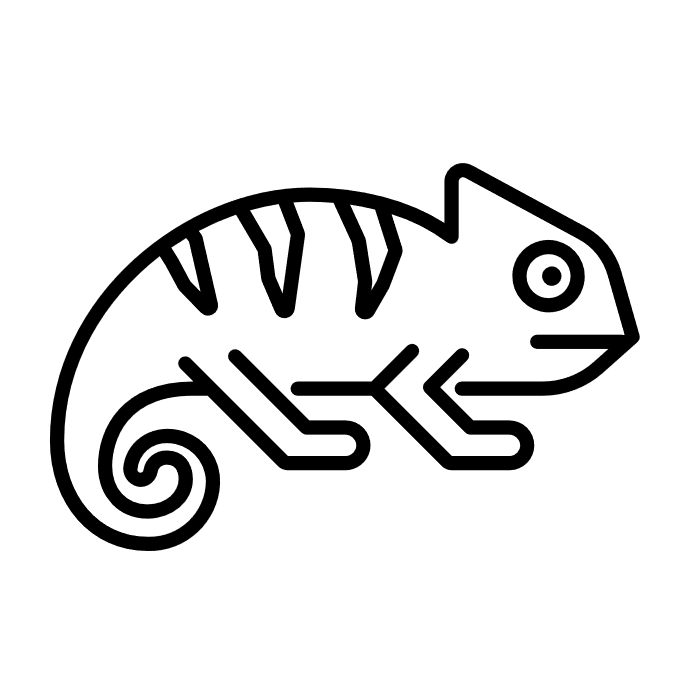
\includegraphics[scale=0.06]{geek.png}\\Davide Difino \& Celina Proffen \\
       \vspace{1.5cm}
       \vfill



        Project in the context of Prof. Ludwig's course: \\
        \textbf{Public Finance in Macroeconomics: Heterogenous Agent Models}\\
        at the Graduate School of Economics, Finance, and Management
       \vspace{0.8cm}
   \end{center}

\newpage

\section{Extension of Code}
\subsection{Embed the code into a general equilibrium model}

Please have a look at the code \textit{Project6\_embed\_in\_GE.m} to find out about our embedment into general equilibrium.

\subsection{Why can an OLG economy be dynamically inefficient?}

An OLG economy might not be (Pareto) efficient in equilibrium if capital output elasticity ($\alpha$) is low. This leads the economy to accumulate more capital than indicated by the "golden rule", that is, the capital stock that maximizes per capita consumption. The reduction of per capita consumption level is given by the fact that the return of capital implied by the capital stock is lower than the growth of the economy. Then, assuming the economy has an infinite time horizon, it would be possible to transfer resources from the future, resulting in a Pareto improvement. \\
Put differently, the golden rule capital stock maximises productive efficiency. If the households of an OLG economy are holding more or less than this capital stock, the economy is dynamically inefficient. In the present case, people save too much individually because they don't know when they will die (and their not consumed money will be burned!!). However, on aggregate, people do die which leads to a too high stock of saved capital and a below optimal rate of return. One possibility to amend this is to insure people such that in the old age they will receive some pension inducing them to save less for old age. This increases r and even makes savings more profitable. \\

\subsection{Calculate the consumption equivalent variation between alternative
policy scenarios}

Please have a look at the code \textit{Project6\_welfare.m} to see our welfare analysis.\\
We received the following output: 

\begin{center}
\begin{tabular}{ |l|l| } 
\hline
Value PE of newborns, orig. pension rule: & -227601.2428\\
\hline
Value PE of newborns, altern. pension rule: & -37.5467\\
\hline
Equivalent variation in PE (tetta $=2$): & -0.99984 \\ % or 6060.8107 if the other way around
\hline
Equilibrium interest rate, orig. pension rule & 0.0036461\\
Equilibrium capital output ratio, orig. pension rule & 6.1628\\
Wage scaling factor, orig. pension rule: & 1.6394\\
Value GE of newborns, orig. pension rule: & -126806.5999\\
\hline
Equilibrium interest rate, altern. pension rule & 0.038479\\
Equilibrium capital output ratio, altern. pension rule & 3.7263\\
Wage scaling factor, altern. pension rule & 1.2813\\
Value GE of newborns, altern. pension rule: & -32.3053\\
\hline
Equivalent variation in GE (tetta $=2$): &  -0.99975 \\ % 3924.2598 if the other way around
\hline
\end{tabular}
\end{center}

The table shows the consumption equivalent variation for the partial as well as for the general equilibrium. Since the value of the orig. pension rule (no pension) is lower than the value of the alternative pension rule (pension, rr$=$0.6) for both, partial and general equilibrium, we know that the alternative rule is advantages, yet, we can not interpret the difference. Using the equivalent variation, we calculated the compensation needed to make an individual indifferent between the two regimes. In line with the comparison of the values (orig. vs. altern.), we see that the equivalent variation is negative, that is, individuals are better off in the alternative regime (with a pension system) and need to pay some money in order to reduce their value to the value they received from the original regime.

\section{Problem 2: Pension Reform in Steady State Comparison}
We make two simplifying assumptions: 
\begin{itemize}
    \item One receives rr * average income of the population as a pension. Therefore, shocks don't matter on aggregate. 
    \item The tax rate (=tau) is the same for every worker.
\end{itemize}

\subsection{How do the welfare consequences depend on risk aversion, tetta?}

$$ g_t = ( \frac{V_t}{\bar{V_t}})^\frac{1}{1-\theta}-1 $$

\begin{center}
\begin{tabular}{ |l|l| } 
\hline
 & tetta = 2 \\ % tetta = 1  \\
\hline
Equivalent variation in PE : & -0.99984 \\ %& \inf  \\ 
\hline
Equivalent variation in GE : &  -0.99975 \\ %& -1  \\ 
\hline
\end{tabular}
\end{center}

$\theta$ is the risk aversion parameter. It defines how strong an individual reacts to uncertainty. If $\theta$ = 1, we have the special case of log utility (here: value). If $\theta > 1$, then the exponent becomes negative. This leads to... . If $0 < \theta < 1$, then the exponent is positive. This leads to... .

% tetta = 1
%Value PE of newborns, orig. pension rule: -15.1924
%Value PE of newborns, altern. pension rule: -8.6896
%Equivalent variation in PE: Inf
%Value GE of newborns, orig. pension rule: -4.148
%Value GE of newborns, altern. pension rule: -4.6683
%Equivalent variation in GE: -1


\subsection{Decompose the welfare effects in partial equilibrium and the remaining general equilibrium effects}
To answer this question, we compare the welfare consequences of a change from the original policy to the alternative policy for partial and general equilibrium. Therefore, we can compare the equivalent variations between the two regimes. The EV of the partial equilibrium is slightly bigger in absolute value than the EV of the general equilibrium, leading to an individual being willing to give up more consumption in order to change from a regime with no pension system to a regime with a pension system (with rr = 0.6). This makes intuitively sense, since the partial equilibrium does not take into account that the interest rate is reacting to behavioural changes and consequently, overestimates the effects of the policy. 

\subsection{Why is it problematic to compare steady states for this type of policy analysis?}
The problem arises from the transition period. Comparing steady state evaluates the policy only after convergence occurred, but it does not take into account that there is a transition period before convergence that might come with different effects for different generations. 

\section{Transitional Dynamics}

\subsection{Detailed write-up that describes how you would implement the solution}

\begin{itemize}
    \item Step 1: Solve model for rr\_init and rr\_final in steady state (as done in problem 2) 
    \item Step 2: Store values
    \begin{itemize}
    \item Store the estimates for r, and call them r\_init and r\_final;
    store the distribution of assets in both steady states and call them PhiAss\_init and PhiAss\_final and Phi\_init and Phi\_final (PhiAss also accounts for the distribution of Assets by shocks, Phi is by age only) 
    \item Store ass\_init and ass\_final
    \item Store grid\_sav\_init and grid\_sav\_final which tells you the nominal amount of savings by cohort dependent on shocks
    \end{itemize}
Remark: \textit{The combination of all this knowledge, will suffice to see how agents at a certain age (and with an associated probability of dying in the future), with a certain asset holding and given a certain shock realization behave $\rightarrow$ from this we hope to derive the savings decision in the previous period by cohort and shock (see Euler equation)}

\item Choose T $=$ 100 \\
\textit{Choose a T, which represents the assumption about the number of periods that it will take to achieve (almost) convergence from the old to the new steady state}

\item Choose M $=$ 100 \\
\textit{This is the number of iterations that we will apply to each interest rate guess to solve for the equilibrium of this interest rate guess}

\item Perform (linear) interpolation and obtain a Tx1 vector of interest rates r\_t\_m between r\_init and r\_final\\
\textit{This is our initial guess for the development of interest rates}

\item	LOOP over $m/M$: \\
\textit{Each iteration will improve the (initially linear) guess of pathways of r over time}
\item Use the linear interpolation from above as initial guess in m$=$1

\begin{itemize}
    \item Compute the wages over age groups \\
\textit{Use the grid of interest rates (“pathways”) to compute the equilibrium wages (es in the GE code from exercise 2)}

\item Find optimal tau\\
\textit{We solve the pension system for the rr-final pension system specification (s.t. government budget constrain is fulfilled)}

\item Solve the household model backwards starting by T-1 (taking T, which is the model under r\_final as given)- loop over t

\begin{itemize}
    \item Transform the vector of assets for the final period to account for the proportion of people dying from the previous age to the next; i.e. take $ass*Phi*(1/1-s)$; then shift everything one period backward s.t. the assets of 80 year old in the final period are now in position 79 of the vector
    \item Then compute for each generation in t the expected value for a\_next period – savings\_next period by aggregating over shocks. 
    Idea is to reach Euler Equation – maybe implement the code I sent on WSP on Latex
    \item Then, applying the Euler equation for each generation 2 up until jr compute assets today for each generation.
    (basically you just rewrite the Euler equation $a\_gen\_today = s\_gen\_tomorrow + u’^(-1){(surv*beta)/(1+r\_guess) \\E $ $[u’(a\_gen+1\_tomorrow – s\_gen+1\_tomorrow)]}$ 
    Note: (The newborns (their asset distribution is calibrated given the income shock realization distribution)\\
    Note, you are using a rate of return now, which differs of that of the initial steady state!
    \item At this point, I am actually a bit confused on how you would do to compute the second iteration... \\
    I guess, that given the initial assets in T-1 which you computed in the last step, you must just solve the standard household model again for each generation. Then, you could repeat the same step as above for all iterations over t, starting with T-2, then T-3, …
    \item Aggregate and store assets across all generations for t 
    The goal here is to get again the overall assets and the distribution which you need for the next loop of t
\end{itemize}
\item	Obtain updated values for r pathway by solving the firm side in each period of time t 
Therefore use the calculated aggregate assets in the economy solve for the rate of return in the GE code
\item Update the guess for the pathway of r at each t \E T
Remember this works by linear interpolation of the old guesses vector and the new one
\end{itemize}
\end{itemize}


\subsection{Make an attempt to implement the solution}

Please have a look at the code \textit{Project6\_transition.m} to find out about our attempt to implement transitional dynamics into our code. 


\section{Literature}
\cite{abbott2019education} develop a heterogenous agents OLG model to assess how financial aid policies act on education, labor and savings decisions of households. It also analyses the welfare effects of policies, concluding that it would be beneficial for society (in this case everything is calibrated to the United States) if more direct financial aid in form of ability-based grants would be handed out to students. 

The agents differ in their “states” and “possible choices” over the life cycle. Young people have to choose their level of education (no high school degree, high school or college) depending on how much education costs in terms of financing and psychic costs. Both are different for agents of different background and with different abilities. In particular, the available loans and grants differ in parents wealth and own abilities; financing options overall are public and private loans, financial aid, their own working activity, in addition to an intra-vivo transfer that students receive from their parents at the beginning of their model life. 

Parents are matched given the man’s and woman’s education and always have two children of the same sex. They care about their children’s direct well-being (altruistic motive) but also directly about their level of education (something like a prestige motive, paternalistic preferences). Their own wealth as well as the financing opportunities of the child determines the inter vivo-transfers they give to their kids. Cognitive and non-cognitive skills are transmitted across generations dependent on parents’ education and skills, and important for the psychic costs of studying (mentioned above) and the labour productivity. 
It is to mention that there are really many levels of heterogeneity amongst agents. Some of them are: Age, gender, initial wealth, cognitive and non-cognitive abilities, education, returns to education and the psychic costs of schooling,

We want to mention some model features which we found particularly interesting:
\begin{itemize}
    \item There is financial markets and risk that is only partially insurable (uninsureable risk: idiosyncratic income risk, risk of being born into a disadvantaged family, risk of marrying someone who is bad for your income, and shocks affecting the psychic costs of eduction)
    \item Agents work and earn, they have gender specific income trends and can co-insure themselves by accounting for the spousal labor supply too
    \item model earnings as a gender-specific stochastic Roy model with a separate process for each education group and dependent on ability
    \item firm side: the aggregate production function depends on inputs from three types of education and allows for imperfect substitutability between males and females of the same skill
    \item economies of scale in household consumption
    \item debt limits vary over the life cycle
\end{itemize}

The model is calibrated with a wide variety of data sources. Amongst them are “the Current Population Survey (CPS), the Panel Study of Income Dynamics, NLSY79 and NLSY97, the National Center for Education Statistics (NCES), the Survey of Consumer Finances (SCF), and the National Accounts“ (see p. 4 of the paper). 

They estimate the model in various stages, and are very careful to explain most steps specifically (sometimes in the Appendix). After exogenously determining some parameters, the first estimations occur in separate calibrations, and the remaining model parameters are estimated in a General Equilibrium context. 
 Examining the model’s implications, the authors find realistic values for intergenerational persistence of income rank and education outcomes. In addition, the life cycle profiles of income and consumption seems plausible. Other variables like wealth and ability are assessed in terms of their intergenerational transmission properties – these are simultaneously interesting ingredients to the educational choices of children and a consistent result w.r.t. to empirical observations. Most of these aspects are analysed by gender, wealth and education level. 
 
Finally, the authors simulate experiments, where e.g. a treatment group of high school graduates receives a subsidy for their college tuition and the rest does not, or where federal loan programs are reduced, etc. They measure how various policy changes would influence welfare (always measured in consumption equivalent variations) and output, and find that in general it is welfare enhancing to increase financial assistance and incentivize education. They identify ability-based grants as the most efficient measure amongst those considered, as it will lead to more high-ability individuals becoming educated parents and again getting more high-ability children. 

\pagebreak

\bibliography{project6.bib}

\pagebreak

\end{document}